

\chapter{Architektur des DeepLabV3+ Modells mit ResNet-50 Backbone}

Das DeepLabV3+ Modell ist eine leistungsstarke Architektur für die semantische Segmentierung von Bildern. In diesem Kapitel werden wir uns näher mit der Architektur des Modells befassen, insbesondere mit dem ResNet-50 Backbone.

\section{Backbone-Netzwerk}
    Das Backbone-Netzwerk ist für die Extraktion aussagekräftiger Merkmale aus dem Eingangsbild verantwortlich. In diesem Fall basiert das Backbone-Netzwerk auf der ResNet-50 Architektur. ResNet-50 ist ein tiefes CNN, das in verschiedenen Computer Vision Aufgaben herausragende Leistung erzielt hat. Es besteht aus mehreren Faltungs­schichten, die in verschiedene Stufen gruppiert sind, wobei Residualverbindungen zwischen ihnen verwendet werden, um das Problem des verschwindenden Gradienten zu lösen. Diese Residualverbindungen ermöglichen es dem Netzwerk, effektiver zu lernen, indem sie Gradienten über Verbindungen mit geringerer Tiefe propagieren.

\section{Prediction-Head}
    Der Prediction-Head nimmt die von dem Backbone-Netzwerk extrahierten Merkmale und generiert die endgültigen Vorhersagen. Im DeepLabV3+ Modell verwendet der Prediction-Head atrous (oder dilatierte) Faltungen mit unterschiedlichen Dilationsraten, um mehrskalige Informationen zu erfassen. Dadurch kann das Modell sowohl detaillierte lokale Informationen als auch Kontextinformationen berücksichtigen.
    
    Das ursprüngliche DeepLabV3+ Modell wird auf dem ImageNet-Datensatz vortrainiert, der Millionen von gelabelten Bildern aus Tausenden von Kategorien enthält. Dieses Vortraining hilft dem Modell, generische visuelle Merkmale zu erlernen, die für spezifische Aufgaben feinabgestimmt werden können.
    
    Im bereitgestellten Code wird das vortrainierte DeepLabV3+ Modell mit dem ResNet-50 Backbone geladen. Das bedeutet, dass das Backbone die anfänglichen Schichten von ResNet-50 umfasst, die für die Merkmalsextraktion verantwortlich sind. Die genauen Schichten und ihre Konfigurationen können recht komplex sein, aber sie beinhalten in der Regel mehrere Faltungsschichten, Pooling-Schichten zur Verkleinerung der Auflösung und Residualverbindungen.
    
    Die Modifikation im Code betrifft die letzte Schicht des Modells, den Klassifizierer. Im ursprünglichen DeepLabV3+ Modell handelt es sich dabei um eine 1x1-Faltungsschicht, die einen Tensor mit den Dimensionen [Batchgröße, Anzahl der Klassen, Höhe, Breite] erzeugt. Die Anzahl der Klassen im Originalmodell beträgt 21, da es auf dem COCO-Datensatz trainiert wurde, der Objekte aus 21 verschiedenen Kategorien enthält.
    
    Im bereitgestellten Code wird die letzte Schicht jedoch durch eine andere 1x1-Faltungsschicht mit einer geänderten Anzahl von Ausgabekanälen ersetzt. Die ursprüngliche Anzahl von Ausgabekanälen beträgt 256, was der Anzahl der vom Backbone-Netzwerk erlernten Merkmale entspricht. In der modifizierten Version des Codes wird jedoch die Anzahl der Ausgabekanäle auf 3 gesetzt, was darauf hinweist, dass das Modell einen Tensor mit den Dimensionen [Batchgröße, 3, Höhe, Breite] ausgibt. Diese Änderung der Anzahl der Ausgabekanäle erfolgt, um das Modell für eine spezifische Aufgabe mit drei Klassen anstelle der ursprünglichen 21 Klassen anzupassen.
    
    Insgesamt handelt es sich bei dem DeepLabV3+ Modell mit ResNet-50 Backbone um eine leistungsstarke Architektur für semantische Segmentierungsaufgaben. Durch die Modifikation der letzten Schicht passt der Code das Modell an, um Pixel in eine von drei Klassen zu klassifizieren.
    
    \textbf{Code-Beispiel:}
    
    \begin{lstlisting}[language=Python]
    Net = torchvision.models.segmentation.deeplabv3_resnet50(pretrained=True)  # Modell laden
    Net.classifier[4] = torch.nn.Conv2d(
        256,
        3,
        kernel_size=(1, 1),
        stride=(1, 1)
    )  # Letzte Schicht auf 3 Klassen ändern
    Net = Net.to(device)
    
    optimizer = torch.optim.Adam(params=Net.parameters(), lr=Learning_Rate)  # Adam-Optimizer erstellen
    \end{lstlisting}
    
\section{Laden des Modells}
    Der Code beginnt damit, das DeepLabV3+ Modell mit ResNet-50 Backbone mithilfe der torchvision-Bibliothek zu laden. DeepLabV3+ ist ein beliebtes Modell für die semantische Segmentierung, d.h., es weist jedem Pixel in einem Eingangsbild eine Klassenbezeichnung zu. Das ResNet-50 Backbone ist ein Typ von Faltungsneuronalem Netzwerk (CNN), das für seine Effektivität bei der Extraktion von Merkmalen aus Bildern bekannt ist.
    
\section{Modifikation der letzten Schicht}
    Anschließend wird die letzte Schicht des geladenen Modells modifiziert. Im Originalmodell ist die letzte Schicht ein Klassifizierer, der eine Wahrscheinlichkeitsverteilung über 21 verschiedene Klassen (wie "Person", "Auto", "Hund", usw.) erzeugt. In diesem Code wird die letzte Schicht jedoch durch eine 1x1-Faltungsschicht ersetzt. Diese Modifikation ändert die Ausgabe des Modells so, dass eine Wahrscheinlichkeitsverteilung über 3 Klassen anstelle von 21 erzeugt wird. Die spezifischen Werte für die Kernelgröße und den Stride bestimmen das Verhalten der Faltung.

\section{Verschieben des Modells auf ein Gerät}
    Das modifizierte Modell wird dann auf ein spezifiziertes Gerät verschoben, das entweder die CPU oder eine GPU sein kann. Dieser Schritt stellt sicher, dass die Berechnungen, die das Modell durchführt, auf dem ausgewählten Gerät durchgeführt werden. Die Nutzung einer GPU kann die Schulung und Inferenz von Deep Learning Modellen erheblich beschleunigen.

\section{Erstellen des Optimierers}
    Ein Optimierer ist ein Algorithmus, der die Parameter des Modells während des Trainingsprozesses anpasst, um die Verlustfunktion zu minimieren. In diesem Code wird ein Adam-Optimierer erstellt, der das Modellparameter (erhalten durch \texttt{Net.parameters()}) und die Lernrate (angegeben durch \texttt{Learning\_Rate}) als Eingabe verwendet. Die Lernrate bestimmt die Schrittgröße, mit der der Optimierer die Modellparameter basierend auf den berechneten Gradienten während der Rückwärtspropagation aktualisiert.
    
    Indem Sie dieser Architektur folgen, haben Sie ein modifiziertes DeepLabV3+ Modell mit ResNet-50 Backbone, das Bilder in eine von drei Klassen segmentieren kann. Die Modellparameter werden während des Trainings mit dem Adam-Optimierer und der angegebenen Lernrate optimiert.



\chapter{Convolutional Neural Network Trainings Prozess}

\section{Was ist Training?}
    Bevor wir uns mit dem Trainingsprozess von Convolutional Neural Networks (CNNs) befassen, ist es sinnvoll, das Konzept des Trainings von neuronalen Netzwerken kurz aufzufrischen. Training bezieht sich auf den Prozess des Anpassens der Gewichte und Bias-Werte eines neuronalen Netzwerks, um eine bestimmte Aufgabe zu erlernen. Im Fall von CNNs besteht das Ziel darin, das Netzwerk auf eine bestimmte Bildklassifizierung oder ein anderes visuelles Erkennungsproblem vorzubereiten.
    
    Der Trainingsprozess ist von entscheidender Bedeutung für die Leistungsfähigkeit von CNNs. Während des Trainings lernt das Netzwerk, relevante Merkmale aus den Trainingsdaten zu extrahieren und Muster zu erkennen. Durch die Optimierung der Gewichte und Bias-Werte kann das Netzwerk lernen, geeignete Entscheidungen zu treffen und präzise Vorhersagen zu treffen.

\section{Trainingsprozess}
    Der Trainingsprozess eines CNNs lässt sich grob in verschiedene Schritte und Phasen unterteilen. Zunächst werden die Trainingsdaten geladen und gegebenenfalls vorverarbeitet, um eine optimale Eingabe für das Netzwerk zu gewährleisten. Dies kann Aufgaben wie das Skalieren der Bilder, das Normalisieren der Daten oder das Anwenden von Data Augmentation-Techniken umfassen.
    Während des Trainingsprozesses werden die Eingabedaten durch das CNN propagiert, wobei die Convolutional-Schichten und Pooling-Schichten verwendet werden, um Merkmale auf verschiedenen Abstraktionsebenen zu extrahieren. Aktivierungsfunktionen wie die ReLU-Funktion werden angewendet, um die Nichtlinearität des Netzwerks zu erhöhen.
    
    Ein entscheidender Schritt ist die Berechnung des Verlusts (Loss), der den Unterschied zwischen den vom Netzwerk vorhergesagten Ausgaben und den tatsächlichen Labels misst. Die Wahl des geeigneten Verlustmaßes hängt von der spezifischen Aufgabe ab, beispielsweise der Kreuzentropie-Verlust für Klassifizierungsaufgaben.
    Um den Verlust zu minimieren und die Gewichte anzupassen, wird der Backpropagation-Algorithmus angewendet. Dabei werden die Gradienten der Verlustfunktion bezüglich der Gewichte berechnet und anschließend mittels eines Optimierungsverfahrens, wie zum Beispiel dem Stochastic Gradient Descent (SGD), verwendet, um die Gewichte in die richtige Richtung zu aktualisieren.
    
    Der Trainingsprozess wird in der Regel über mehrere Epochen durchgeführt, wobei jede Epoche eine Durchlauf der gesamten Trainingsdaten umfasst. Dies ermöglicht es dem Netzwerk, schrittweise zu lernen und seine Leistung zu verbessern. Es ist auch üblich, das Netzwerk regelmäßig auf einem separaten Validierungsdatensatz zu testen, um die Überanpassung (Overfitting) zu vermeiden.

\section{Stochastic Gradient Descent (SGD)}
    Der Stochastic Gradient Descent\footfullcite{amari1993backpropagation} (SGD) ist ein Optimierungsverfahren, das eine zentrale Rolle im Trainingsprozess von CNNs spielt. Im Gegensatz zum Gradientenabstiegsverfahren (Gradient Descent), bei dem der Verlust über den gesamten Trainingsdatensatz berechnet wird, verwendet SGD eine zufällige Teilmenge der Daten, um den Gradienten zu approximieren.
    
    Der Einsatz von SGD hat mehrere Vorteile. Erstens ermöglicht er eine schnellere Berechnung des Gradienten, da nur eine Teilmenge der Daten betrachtet wird. Zweitens macht die zufällige Auswahl der Daten das Verfahren robuster gegenüber lokalen Minima, da das Netzwerk unterschiedliche Datenmuster im Verlauf des Trainingsprozesses betrachtet.
    
    \begin{figure}[h]
        \centering
        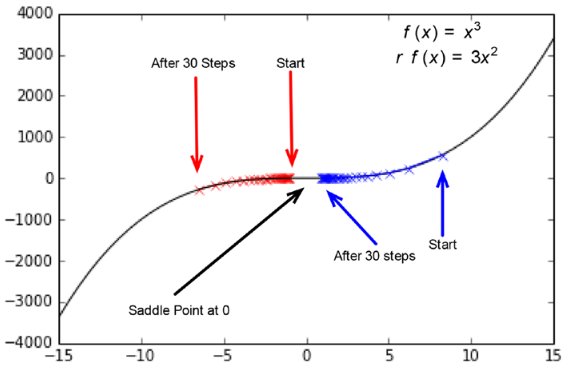
\includegraphics[width=0.8\textwidth]{img/gradient_descent.png}
        \caption{Beispiel von Stochastic Gradient Descent mit 30 Lernschriten.}
        \label{fig:Stochastic_Gradient_Descent}
    \end{figure}
    
    Die Anpassung der Lernrate ist ein wichtiger Aspekt im SGD-Algorithmus. Die Lernrate bestimmt die Größe der Aktualisierungen der Gewichte und beeinflusst somit die Konvergenzgeschwindigkeit des Netzwerks. Eine zu hohe Lernrate kann zu instabilen oder schlecht konvergierenden Lösungen führen, während eine zu niedrige Lernrate den Trainingsprozess verlangsamen kann. Es ist daher oft erforderlich, die Lernrate im Laufe des Trainings anzupassen, beispielsweise durch den Einsatz von Lernrateplanern oder adaptiven Methoden wie Adam.

\section{Backpropagation}
    Backpropagation\footfullcite{amari1993backpropagation} ist ein wesentlicher Bestandteil des Trainingsprozesses von neuronalen Netzwerken, einschließlich CNNs. Es handelt sich um ein Verfahren zur Berechnung der Gradienten der Verlustfunktion bezüglich der Gewichte des Netzwerks.
    
    Der Backpropagation-Algorithmus funktioniert, indem er die Fehlerinformationen vom Ausgabeneuron zurück durch das Netzwerk propagiert. Dabei werden die partiellen Ableitungen der Verlustfunktion nach den Gewichten in den Schichten berechnet. Dies ermöglicht es, den Gradienten des Verlusts bezüglich der Gewichte zu bestimmen und somit die Gewichte entsprechend anzupassen.
    
    Dank der effizienten Berechnung des Backpropagation-Algorithmus ist es möglich, CNNs mit vielen Schichten zu trainieren. Die Gradienten werden schichtweise berechnet, wodurch eine effektive Ausbreitung der Fehler ermöglicht wird. Dieser Prozess des Gradientenabstiegs ermöglicht es dem Netzwerk, seine Gewichte so anzupassen, dass der Verlust minimiert wird.

\section{Hyperparameter-Tuning}
    Hyperparameter\footfullcite{mantovani2016hyper} sind Parameter, die nicht direkt aus den Daten gelernt werden, sondern vor dem Trainingsprozess festgelegt werden müssen. Sie haben einen erheblichen Einfluss auf die Leistungsfähigkeit des CNNs und müssen sorgfältig ausgewählt werden.
    
    Das Tuning von Hyperparametern beinhaltet die Suche nach den besten Werten für diese Parameter, um eine optimale Leistung des CNNs zu erzielen. Dies kann durch manuelles Ausprobieren verschiedener Hyperparameterkombinationen oder durch den Einsatz von automatisierten Methoden wie Grid Search oder Bayesian Optimization erfolgen\footfullcite{amari1993backpropagation}.
    
    \begin{figure}[h]
        \centering
        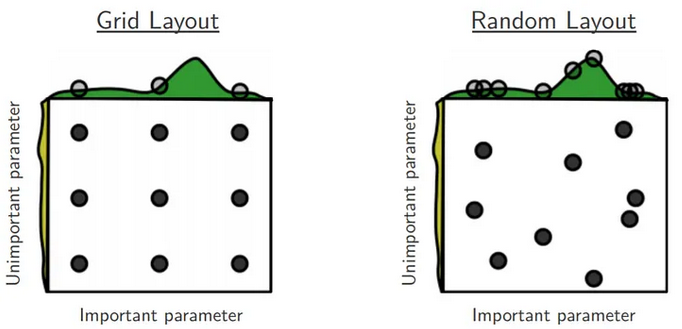
\includegraphics[width=\textwidth]{img/hyperparameter_tuning.png}
        \caption{Hyperparameter tuning.}
        \label{fig:hyperparameter_tuning}
    \end{figure}
    
    Beispiele für Hyperparameter sind die Lernrate, die Anzahl der Schichten und Filter im Netzwerk, die Größe des Mini-Batches, die Dropout-Rate und die Regularisierungsparameter. Das richtige Tuning dieser Hyperparameter kann dazu beitragen, eine bessere Generalisierungsfähigkeit des Netzwerks zu erreichen und Überanpassung zu vermeiden.

\section{Regularisierungstechniken}
    Regularisierungstechniken\footfullcite{ghiasi2018dropblock} sind Methoden, die während des Trainingsprozesses angewendet werden, um die Überanpassung des Netzwerks an die Trainingsdaten zu reduzieren und die allgemeine Leistungsfähigkeit zu verbessern.
    
    Eine gängige Regularisierungstechnik ist die L1- und L2-Regularisierung\footfullcite{ibrahim2023anomaly}, bei der ein Regularisierungsterm zur Verlustfunktion hinzugefügt wird, der die Gewichte des Netzwerks beeinflusst. Dies hilft, die Gewichte zu reduzieren und die Modellkomplexität zu verringern.
    
    Ein weiteres Regularisierungsverfahren ist Dropout\footfullcite{labach2019survey}, bei dem während des Trainings zufällig einige Neuronen deaktiviert werden. Dadurch wird das Netzwerk gezwungen, redundante Merkmale zu lernen und erhöht die Robustheit gegenüber Überanpassung.
    
    Data Augmentation ist eine weitere Regularisierungstechnik, bei der die Trainingsdaten künstlich erweitert werden, indem sie transformiert oder mit Rauschen versehen werden. Dies ermöglicht es dem Netzwerk, mehr Variationen der Daten zu sehen und generalisierbarere Merkmale zu lernen.
    
    Die Anwendung von Regularisierungstechniken während des Trainingsprozesses trägt dazu bei, die Leistungsfähigkeit des CNNs zu verbessern und die Überanpassung an die Trainingsdaten zu reduzieren.
